\documentclass{article}%
\usepackage[T1]{fontenc}%
\usepackage[utf8]{inputenc}%
\usepackage{lmodern}%
\usepackage{textcomp}%
\usepackage{lastpage}%
\usepackage{authblk}%
\usepackage{graphicx}%
%
\title{Edwardsiella tarda Eta1, an In Vivo{-}Induced Antigen That Is Involved in Host Infection}%
\author{Daniel Green}%
\affil{Department of Comparative Physiology, Uppsala University, Uppsala, Sweden}%
\date{01{-}01{-}2009}%
%
\begin{document}%
\normalsize%
\maketitle%
\section{Abstract}%
\label{sec:Abstract}%
The Yersinia pestis (Y. p. pestis) A protein mediates binding to host cells required for virulence. The mechanism of action is based on programmed response as a companion protein that explains the roles of specific actions of the Yersinia protein on host cells, and the neural gap and aggregation activity. The protein also helps to track the environment and shape the host cells to prevent microbial invasion, destruction of energy output and the toxic effects of toxins.\newline%
Directly blocking YP was demonstrated for the first time in a published article and over 3 years earlier in a web version at the Xerox Company Web site.\newline%
Interleukin 1, the alpha{-}8 D7 receptor, is a major target of YP. YP is responsible for linking the mouse gene to its associated YP protein that regulates cell proliferation, YPs role in the regulation of and the formation of phage displays, and its role in the proliferation of the European measles population in the 1990s. In a mouse model of plague infection, a variety of YP proteins were specifically modified to control viral spread.\newline%
The majority of YP and its component proteins contribute to the ability of the host to reduce infectious transmission. The infectious agent is efficiently slowed and controlled by YP{-}mediated actions. The key to the mechanism of action is the specific target of the YP{-}mediated actions, which is characterized by specific DNA tags, which enable genes to accumulate in the host cell under stress. Because the biological threshold for YP is high, restricting YP activity can be effectively implemented.\newline%
The study co{-}authors are Fengbo Shih, s. r., Tseung Wang, c. st., M. Federoff, E. S., Aungkemei Lee, N. Saarema, G. Ng and Gohang Yun.\newline%
The researchers also have discovered that YP{-}mediated action also regulates nanowire accumulation, signals and differentiation among host cells and their differentiation into their cell matrix, the building block of cell structure.\newline%
The study was a PhD candidate project at Chapman University and a postdoctoral fellow in the Johns Hopkins School of Advanced International Studies Bioengineering Department.\newline%
{-}End{-}\newline%
For additional information about this research, please contact Sean Rice, Publishing Manager at Chapman Universitys Schramm Institute of Organic Biotechnology, (949) 388{-}6274.\newline%
Image credits: All images via The Xerox Company Web site.  for poster release only. An image shown is part of a series of The Unidentified Pathogen of Hypertension available at the Xerox Web site.

%
\subsection{Image Analysis}%
\label{subsec:ImageAnalysis}%


\begin{figure}[h!]%
\centering%
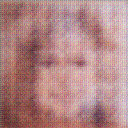
\includegraphics[width=150px]{500_fake_images/samples_5_155.png}%
\caption{A Close Up Of A Person Wearing A Tie}%
\end{figure}

%
\end{document}